\documentclass[10pt, oneside]{article}

\usepackage{amsmath}
\usepackage{amsthm}
\usepackage{amssymb}
\usepackage{calrsfs}
\usepackage{wasysym}
\usepackage{verbatim}
\usepackage{bbm}
\usepackage{color}
\usepackage{graphics}
\usepackage{geometry}
\usepackage{graphicx}

% for tables
\usepackage{booktabs}
% \usepackage{multirow}
% \usepackage{siunitx}

% \usepackage{natbib} % For bibliography management
\usepackage[numbers]{natbib}
\usepackage{hyperref} % For clickable references

\geometry{tmargin=.75in, bmargin=.75in, lmargin=.75in, rmargin = .75in}  

\newcommand{\R}{\mathbb{R}}
\newcommand{\C}{\mathbb{C}}
\newcommand{\Z}{\mathbb{Z}}
\newcommand{\N}{\mathbb{N}}
\newcommand{\Q}{\mathbb{Q}}
\newcommand{\Cdot}{\boldsymbol{\cdot}}

\newtheorem{thm}{Theorem}
\newtheorem{defn}{Definition}
\newtheorem{conv}{Convention}
\newtheorem{rem}{Remark}
\newtheorem{lem}{Lemma}
\newtheorem{cor}{Corollary}

\title{System-2 Course: Session 4
\\ Neuro-Symbolic VQA: Disentangling Reasoning from Vision and Language Understanding
}
\author{Farzan Rahmani - 403210725}
\date{Spring 2025}

\begin{document}

\maketitle

\tableofcontents

\pagebreak

\section{Introduction}

\begin{rem}
This lecture note provides a comprehensive overview of Neuro-Symbolic Visual Question Answering (VQA), drawing upon the lecture slides of the course "CS 957, System-2 AI", the paper "Neural-Symbolic VQA: Disentangling Reasoning from Vision and Language Understanding" by \citet{Yi2018}, and the paper "CLEVR: A Diagnostic Dataset for Compositional Language and Elementary Visual Reasoning" by \citet{Johnson2017a}. This approach emphasizes the separation of perception and reasoning for more robust and interpretable VQA systems.
\end{rem}
Some examples of the VQA task are in Figure \ref{fig:f1} which need to be answered in natural language text.

\begin{figure}
    \centering
    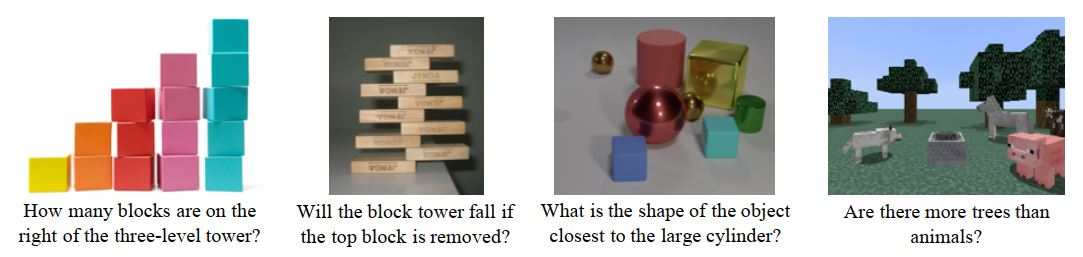
\includegraphics[width=0.8\linewidth]{Fig1.JPG}
    \caption{Human reasoning is interpretable and disentangled: we first draw abstract knowledge of
    the scene via visual perception and then perform logic reasoning on it. This enables compositional,
    accurate, and generalizable reasoning in rich visual contexts.}
    \label{fig:f1}
\end{figure}

\section{The CLEVR Diagnostic Dataset}
The CLEVR dataset plays a crucial role in evaluating and understanding the capabilities of VQA systems, including neuro-symbolic ones. A field guide to the CLEVR dataset is depicted in the Figure \ref{fig:f2}.

\subsection{Motivation}
\begin{itemize}
    \item Existing VQA benchmarks often contain biases that models can exploit without performing true visual reasoning.
    \item They conflate multiple sources of error.
    \item CLEVR was designed as a diagnostic dataset to test a range of visual reasoning abilities with minimal biases and detailed annotations.
    \item The name is a homage to Clever Hans, illustrating the danger of systems superficially solving tasks.
\end{itemize}

\subsection{Design Principles}
\begin{itemize}
    \item Synthetic Images of Simple 3D Shapes: This simplifies recognition and allows a focus on reasoning skills.
    \item Complete and Exclusive Information: Each image contains all necessary information, preventing reliance on external knowledge.
    \item Minimized Question-Conditional Bias: Rejection sampling within question families helps avoid biases.
    \item Structured Ground-Truth Representations: Images are annotated with object positions and attributes, and questions are represented as functional programs. These programs, built from basic functions enable in-depth analysis of required reasoning abilities.
    \item Complex Questions Requiring Reasoning: While images are simple, the automatically generated questions are complex, testing counting, comparison, logical reasoning, and memory.
\end{itemize}

\begin{figure}
    \centering
    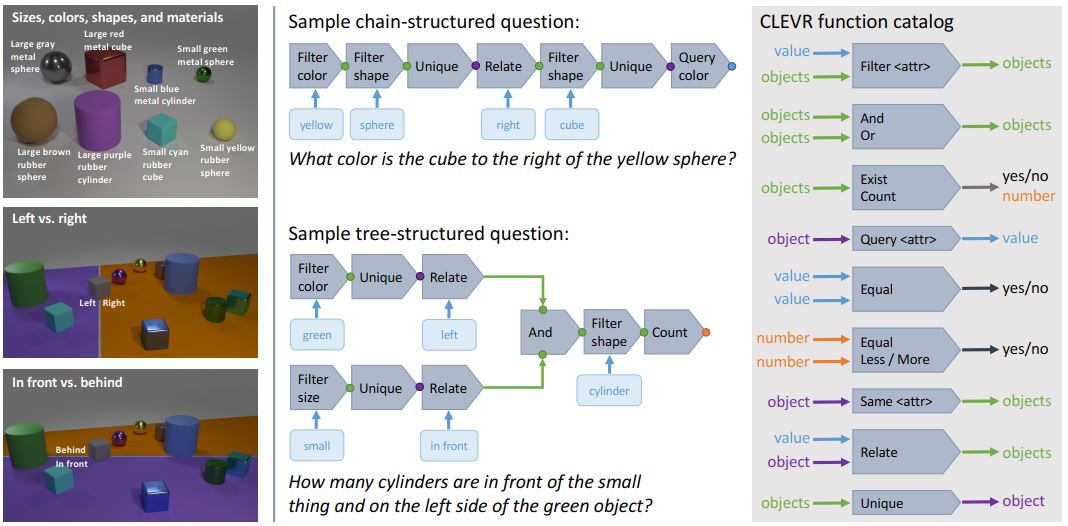
\includegraphics[width=0.9\linewidth]{Fig2.JPG}
    \caption{A field guide to the CLEVR universe. Left: Shapes, attributes, and spatial relationships. Center: Examples of questions and
    their associated functional programs. Right: Catalog of basic functions used to build questions.}
    \label{fig:f2}
\end{figure}

\subsection{Dataset Statistics}
\begin{itemize}
    \item CLEVR contains 100k rendered images and about one million automatically-generated questions, of which 853k are unique.
    \item Questions are categorized by type based on the outermost function in their program (e.g., query-color, exist, count).
    \item Question lengths are generally longer than in other VQA datasets.
\end{itemize}

\subsection{Analysis of VQA Models on CLEVR}
The CLEVR paper \citep{Johnson2017a} analyzes various modern VQA systems, revealing weaknesses. For example, models struggle with:
\begin{itemize}
    \item Short-term memory: Required for attribute comparison and integer equality questions.
    \item Compositional reasoning: Recognizing novel attribute combinations.
    \item Long reasoning chains: Questions with large effective sizes and many spatial relationships.
    \item Spatial relationships: Often relying on absolute image position rather than true relational understanding.
    \item Question topology: Tree-structured questions can be more challenging than chain-structured ones.
\end{itemize}

The concept of effective question size was introduced to show that models struggle with genuinely long reasoning chains, even if shorter sub-programs can sometimes yield the correct answer.

The analysis also highlights cases where models show success, such as spatial attention aiding in identifying object attributes.

\section{Core Idea: Disentangling Perception from Reasoning}
The fundamental principle of Neuro-Symbolic VQA is to separate the visual and linguistic understanding from the logical reasoning process required to answer questions about images. This contrasts with end-to-end neural network approaches where these processes are implicitly learned and often intertwined. The motivation stems from the human ability to reason abstractly once a scene is perceived and a question is understood. We go deeper about this idea and explain how it is possible to disentangle perception from reasoning in the following sections.

\section{Architecture Overview}

\begin{figure}
    \centering
    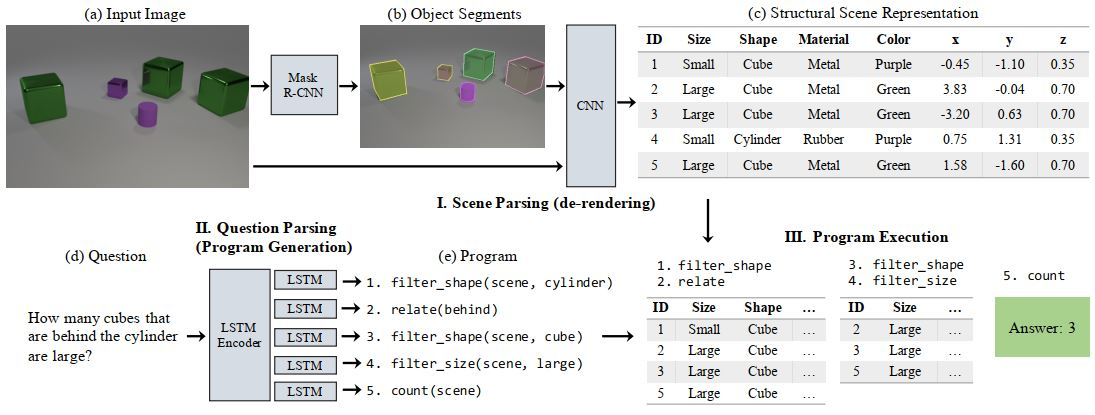
\includegraphics[width=0.9\linewidth]{Fig3.JPG}
    \caption{The model has three components: first, a scene parser (de-renderer) that segments an input
    image (a-b) and recovers a structural scene representation (c); second, a question parser (program
    generator) that converts a question in natural language (d) into a program (e); third, a program
    executor that runs the program on the structural scene representation to obtain the answer.}
    \label{fig:f3}
\end{figure}

The NS-VQA system employs a modular architecture with three main components as you can see in Figure \ref{fig:f3}:

\subsection{Scene Parser (De-renderer)}
This module aims to create a structural, object-based representation of the visual scene.
\begin{itemize}
    \item It begins by generating object segment proposals using Mask R-CNN. Proposals with a bounding box score less than 0.9 are discarded.
    \item For each segment, the network predicts categorical labels of discrete intrinsic attributes such as color, material, size, and shape.
    \item Each object segment, paired with the original image (resized to 224x224), is fed into a ResNet-34 network to extract spatial attributes like pose and 3D coordinates. The inclusion of the original image provides contextual information.
    \item The scene parsing module's object proposal network (Mask R-CNN) uses a ResNet-50 FPN backbone.
    \item The feature extraction network for continuous attributes is trained on the proposed object segments using mean square error as the loss function.
    \item Training of both networks within the scene parser is performed on 4,000 generated CLEVR images for 30,000 iterations with learning rate 0.002 a batch size of 8 for Mask R-CNN and 50 for the feature extraction network.
    \item The output is a disentangled, compact, and rich structural scene representation, detailing each object with its attributes and 3D coordinates.
\end{itemize}

\subsection{Question Parser (Program Generator)}
This module is responsible for converting the natural language question into a latent, hierarchical program.
\begin{itemize}
    \item It utilizes an attention-based sequence-to-sequence (seq2seq) model with an encoder-decoder structure. This type of model is commonly used for mapping one sequence (the question) to another sequence (the program). The lecture slides also mention an Attention-based Bidirectional LSTM.
    \item The encoder is a bidirectional LSTM that processes the input question using jointly trained word embeddings.
    \item The decoder is another LSTM that generates the program tokens sequentially, using an attention mechanism to focus on relevant parts of the encoded question.
    \item The output is a sequence of tokens representing a functional program, where each token corresponds to a specific operation on the scene representation.
\end{itemize}

\subsection{Program Executor}
This module takes the symbolic program generated by the question parser and executes it on the structural scene representation produced by the scene parser to obtain the final answer.
\begin{itemize}
    \item The executor is implemented as a collection of deterministic, generic functional modules in Python.
    \item These modules correspond one-to-one with the tokens in the program sequence.
    \item These modules perform purely symbolic operations on their inputs throughout the execution process.
    \item The program typically starts with a scene token, representing the initial scene representation, and subsequent modules operate on the output of the previous one.
    \item If a type mismatch occurs between the input and output of adjacent modules, an error flag is raised, and the model randomly samples an answer.
    \item Examples of these functional modules include set operations (e.g., filter, unique, union, intersect, count), boolean operations (e.g., equal\_color, greater\_than, exist), query operations (e.g., query\_color, query\_shape), and relation operations (e.g., relate\_front, same\_color).
\end{itemize}

\section{Question Parser Architecture Details}

\subsection{Encoder (Bidirectional LSTM)}
The encoder's role is to take the input question and convert it into a set of encoded vectors that capture the meaning of the question. The NS-VQA system uses a bidirectional LSTM for this purpose.
\begin{itemize}
    \item A Long Short-Term Memory (LSTM) network is a type of recurrent neural network (RNN) capable of learning long-range dependencies in sequential data. It maintains a hidden state that is updated as it processes the input sequence.
    \item A bidirectional LSTM processes the input sequence in two directions: forward and backward. This allows it to consider the context of a word from both the words that precede it and the words that follow it.
\end{itemize}

The input to the encoder is a question of variable length. Each word in the question ($x_i$) is first converted into a word embedding ($\Phi_E\left(x_i\right)$), which is a vector representation of the word learned during training.

The forward LSTM processes the sequence from the first word to the last, producing an output ($e_i^F$) and a hidden vector ($h_i^F$) at each time step $i$:
\begin{equation}
    e_i^F,h_i^F=\mathrm{LSTM}\left(\Phi_E\left(x_i\right),h_{i-1}^F\right)
\end{equation}

Similarly, the backward LSTM processes the sequence from the last word to the first, producing an output ($e_i^B$) and a hidden vector ($h_i^B$) at each time step $i$:
\begin{equation}
    e_i^B,h_i^B=\mathrm{LSTM}\left(\Phi_E\left(x_i\right),h_{i+1}^B\right)
\end{equation}

The encoded vector ($e_i$) at each time step $i$ is then formed by concatenating the forward and backward LSTM outputs:
\begin{equation}
    e_i=\left[e_i^F,e_i^B\right]
\end{equation}

\subsection{Decoder (LSTM with Attention)}
The decoder's role is to generate the output program sequence based on the encoded representation of the question. The NS-VQA system uses an LSTM with an attention mechanism for this.
\begin{itemize}
    \item The decoder is also an LSTM that generates a hidden state ($q_t$) at each time step $t$, based on the previous output token ($y_{t-1}$) and its embedding ($\Phi_D\left(y_{t-1}\right)$):
    \begin{equation}
        q_t=\mathrm{LSTM}\left(\Phi_D\left(y_{t-1}\right)\right)
    \end{equation}
    \item The attention mechanism allows the decoder to focus on the most relevant parts of the encoded input question when generating each token of the output program. It computes a context vector ($c_t$) as a weighted sum of the encoded states ($e_i$) from the encoder. The weights ($\alpha_{ti}$) indicate the importance of each encoded state for the current decoding step.
\end{itemize}

The attention weights are calculated as follows:
\begin{equation}
    \alpha_{ti}\propto\exp{\left(q_t^TW_Ae_i\right)}
\end{equation}
where $W_A$ is an attention weight matrix. For simplicity, the paper \cite{Yi2018} mentions setting the dimensions of $q_t$ and $e_i$ to be the same and $W_A$ to be an identity matrix, which simplifies the weight calculation to:
\begin{equation}
    \alpha_{ti}\propto\exp{\left(q_t^Te_i\right)}
\end{equation}

The context vector ($c_t$) is then computed as the weighted sum of the encoded vectors:
\begin{equation}
    c_t=\sum_{i}{\alpha_{ti}e_i}
\end{equation}

Finally, the context vector ($c_t$) is concatenated with the decoder's hidden state ($q_t$) and passed through a fully connected layer with a softmax activation function to produce a probability distribution over the next token ($y_t$) in the output program sequence:
\begin{equation}
    y_t\sim\mathrm{softmax}\left(W_O\left[q_t,c_t\right]\right)
\end{equation}
where $W_O$ is a weight matrix for the output layer.

The encoder and decoder in the NS-VQA question parser both have two hidden layers with a 256-dimensional hidden vector, and the word vectors have a dimension of 300.

\section{Training the Modules}
The training process involves distinct steps for the scene parser and the question parser:

\subsection{Scene Parser Training}
\begin{itemize}
    \item The Mask R-CNN is trained on rendered images and object masks.  For CLEVR, since original masks weren't available, they were generated using the CLEVR dataset generation tool.
    \item The bounding-box classifier contains 48 classes representing combinations of intrinsic attributes.
    \item The feature extraction CNN is trained using segment-label pairs, where each segment is concatenated with the original image.
    \item Training details (iterations, learning rate, batch size) were mentioned earlier in section 4.
\end{itemize}

\subsection{Question Parser Training}
A two-step procedure is adopted:
\begin{itemize}
    \item Pre-training (Supervised): The question parser is initially trained on a small number of ground truth question-program pairs. The slides mention $\sim$100-300 pairs for 20,000 iterations with a learning rate of $7 \times 10^{-4}$. This teaches the parser to map questions to programs. The NS-VQA paper \cite{Yi2018} specifies using 90, 180, or 270 programs, uniformly drawn from the 90 question families of CLEVR, for pretraining.
    \item Post-training (Reinforcement Learning): The pre-trained parser is then fine-tuned using a larger set of question-answer pairs. The reward is 1 if the executed program gives the correct answer, and 0 otherwise. The REINFORCE algorithm is used for optimization, maximizing the expected return over a constant baseline with a decay weight of 0.9. This stage runs for at most 2 million iterations with early stopping and a learning rate of $10^{-5}$. The batch size is fixed at 64 for both stages. The lecture slides highlight REINFORCE's sample efficiency (both in pre-training and post-training). You can refer to Figure \ref{fig:f4} for more details about efficiency. 
\end{itemize}

\begin{figure}
    \centering
    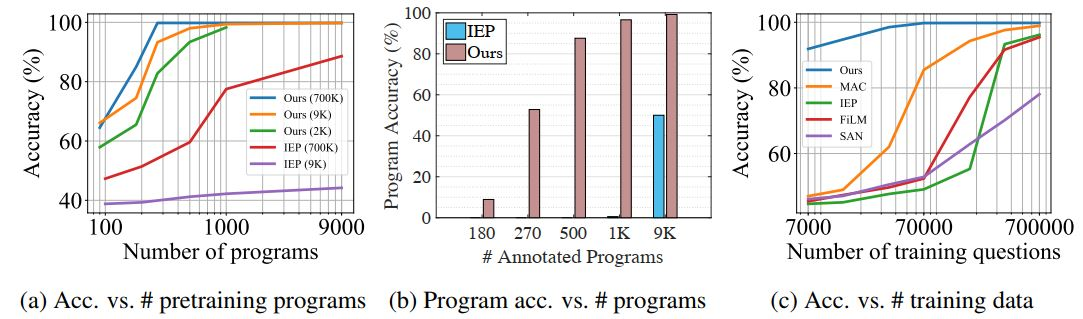
\includegraphics[width=0.9\linewidth]{Fig4.JPG}
    \caption{The model exhibits high data efficiency while achieving state-of-the-art performance and
    preserving interpretability. (a) QA accuracy vs. number of programs used for pretraining; different
    curves indicate different numbers of question-answer pairs used in the REINFORCE stage. (c) QA
    accuracy vs. total number of training question-answer pairs; our model is pretrained on 270 programs.}
    \label{fig:f4}
\end{figure}

\section{REINFORCE Algorithm Details}
\label{sec:reinforce}

\subsection{Question Parser Training}
The training process consists of two phases:

\begin{itemize}
    \item \textbf{Pre-training}: Supervised learning with $\sim$100-300 question-program pairs for 20,000 iterations
    \item \textbf{Post-training}: Reinforcement learning with $\sim$9k-700k question-answer pairs for up to 2 million iterations (with early stopping)
    \begin{itemize}
        \item Reward function: $R = \begin{cases} 
        1 & \text{if program execution yields correct answer} \\
        0 & \text{otherwise}
        \end{cases}$
        \item Training algorithm: REINFORCE policy gradient method
    \end{itemize}
\end{itemize}

\subsection{REINFORCE Fundamentals}
The REINFORCE algorithm optimizes the expected return $J(\theta)$:

\begin{equation}
    \theta^{\star} = \arg \max_{\theta} J(\theta) = \arg \max_{\theta} \mathbb{E}_{\tau \sim p_{\theta}(\tau)} \left[ \sum_{t} r(\mathbf{s}_{t}, \mathbf{a}_{t}) \right]
\end{equation}

Where the expected return can be expressed as:

\begin{equation}
    J(\theta) = \mathbb{E}_{\tau \sim p_{\theta}(\tau)} [r(\tau)] = \mathbb{E}_{\tau \sim p_{\theta}(\tau)} [\sum_{t=1}^{T} r(\mathbf{s}_{t}, \mathbf{a}_{t})] = \int p_{\theta}(\tau) r(\tau) d\tau
\end{equation}

\subsection{Gradient Derivation}
The policy gradient is derived as follows:

\begin{align}
    \nabla_{\theta} J(\theta) &= \int \nabla_{\theta} p_{\theta}(\tau) r(\tau) d\tau \\
    &= \int \frac{p_{\theta}(\tau)}{p_{\theta}(\tau)} \nabla_{\theta} p_{\theta}(\tau) r(\tau) d\tau \\
    &= \int p_{\theta}(\tau) \frac{\nabla_{\theta} p_{\theta}(\tau)}{p_{\theta}(\tau)}  r(\tau) d\tau \\
    &= \int p_{\theta}(\tau) \nabla_{\theta} \log p_{\theta}(\tau) r(\tau) d\tau \quad \text{(Likelihood ratio trick)} \\
    &= \mathbb{E}_{\tau \sim p_{\theta}(\tau)} \left[ \nabla_{\theta} \log p_{\theta}(\tau) r(\tau) \right]
\end{align}

\subsection{Trajectory Probability}
The probability of a trajectory $\tau$ (a program generated by LSTM) under policy $\pi_\theta$ is:

\begin{equation}
    p_{\theta}(\tau) = p(\mathbf{s}_{1})\prod_{t=1}^{T}\pi_{\theta}(\mathbf{a}_{t}|\mathbf{s}_{t})p(\mathbf{s}_{t+1}|\mathbf{s}_{t},\mathbf{a}_{t})
\end{equation}

Taking the logarithm:

\begin{equation}
    \log p_{\theta}(\tau) = \log p(\mathbf{s}_{1}) + \sum_{t=1}^{T} \log \pi_{\theta}(\mathbf{a}_{t} \mid \mathbf{s}_{t}) + \log p(\mathbf{s}_{t+1} \mid \mathbf{s}_{t}, \mathbf{a}_{t})
\end{equation}

\subsection{Final Gradient Expression}

\begin{equation}
    \nabla_{\theta} J(\theta) = E_{\tau \sim p_{\theta}(\tau)} \left[ \nabla_{\theta} \log p_{\theta}(\tau) r(\tau) \right]
\end{equation}

\begin{equation}
    \nabla_{\theta} J(\theta) = E_{\tau \sim p_{\theta}(\tau)} \left[ \nabla_{\theta}\left[\log p(s_{1})+\sum_{t=1}^{T}\log \pi_{\theta}(a_{t}|s_{t})+\log p(s_{t+1}|s_{t},a_{t})\right] r(\tau) \right]
\end{equation}

Since initial state and dynamics are independent of $\theta$:

\begin{equation}
    \nabla_{\theta} J(\theta) = \mathbb{E}_{\tau \sim p_{\theta}(\tau)} \left[ \left( \sum_{t=1}^{T} \nabla_{\theta} \log \pi_{\theta}(\mathbf{a}_{t} \mid \mathbf{s}_{t}) \right) \left( \sum_{t=1}^{T} r(\mathbf{s}_{t}, \mathbf{a}_{t}) \right) \right] \\
\end{equation}

\subsection{Monte Carlo Implementation}
In practice, we approximate the expectation using $N$ samples:

\begin{equation}
    \nabla_{\theta} J(\theta) \approx \frac{1}{N} \sum_{i=1}^{N} \left( \sum_{t=1}^{T} \nabla_{\theta} \log \pi_{\theta}(\mathbf{a}_{i,t} \mid \mathbf{s}_{i,t}) \right) \left( \sum_{t=1}^{T} r(\mathbf{s}_{i,t}, \mathbf{a}_{i,t}) \right)
\end{equation}

\subsection{Parameter Update}
The parameters are updated via gradient ascent:

\begin{equation}
    \theta \leftarrow \theta + \alpha \nabla_{\theta} J(\theta)
\end{equation}

Where $\alpha$ is the learning rate ($10^{-5}$ in NS-VQA).

\subsection{Algorithm Steps}
The complete REINFORCE algorithm:

\begin{enumerate}
    \item \textbf{Sample trajectories}: Generate programs $\{\tau^i\}$ by running current policy $\pi_\theta$
    \item \textbf{Compute rewards}: Execute programs to obtain rewards $r(\tau^i) = \sum_t r(s_i^t,a_i^t)$
    \item \textbf{Estimate gradient}:
    \[
    \nabla_{\theta} J(\theta) \approx \sum_{i} \left( \sum_{t} \nabla_{\theta} \log \pi_{\theta}(\mathbf{a}_{t}^{i} \mid \mathbf{s}_{t}^{i}) \right) \left(\sum_t r(s_i^t,a_i^t)\right)
    \]
    \item \textbf{Update parameters}:
    \[
    \theta \leftarrow \theta + \alpha \nabla_{\theta} J(\theta)
    \]
\end{enumerate}

\begin{rem}
In essence, REINFORCE encourages the question parser to generate programs that lead to correct answers by increasing the probability of successful programs and decreasing the probability of unsuccessful ones, based on the reward signal received after executing the generated program. The process involves sampling programs, executing them, and then updating the parser's parameters based on the outcome. The sample efficiency of REINFORCE in both pre-training and post-training phases is a key characteristic.
\end{rem}


\subsection{Variance Reduction}
To reduce variance in gradient estimates:

\begin{equation}
    \nabla_{\theta} J(\theta) \approx \frac{1}{N} \sum_{i=1}^{N} \left( \sum_{t=1}^{T} \nabla_{\theta} \log \pi_{\theta}(\mathbf{a}_{i,t} \mid \mathbf{s}_{i,t}) \right) (r(\tau^i) - b)
\end{equation}

Where $b$ is a baseline (constant baseline with decay weight 0.9 in NS-VQA).

\begin{rem}
The REINFORCE algorithm follows the general reinforcement learning paradigm:
\begin{itemize}
    \item Generate samples by running the current policy
    \item Estimate returns from experience
    \item Improve the policy using gradient ascent
\end{itemize}
This approach is particularly effective in NS-VQA due to the deterministic nature of program execution, which provides clear reward signals.
\end{rem}

\section{Key Advantages and Results}
The neuro-symbolic approach offers several advantages:

\subsection{Robustness to Long Program Traces and Complex Reasoning}
Executing programs on a symbolic space is more robust to long sequences of reasoning steps compared to purely neural models. This allows the model to solve complex reasoning tasks more effectively, achieving a near-perfect accuracy of 99.8\% on the CLEVR dataset when trained with 270 pretraining programs.

\subsection{Data and Memory Efficiency}
The model performs well even after learning on a small number of training data. Furthermore, the compact structural image representation requires significantly less storage (less than 100 bytes per image) compared to storing original images or feature maps in attention-based methods (at least 20KB per image).

\subsection{Transparency and Interpretability}
The use of symbolic scene representations and program traces provides full transparency to the reasoning process. Each execution step can be interpreted and diagnosed, allowing for a deeper understanding of how the model arrives at an answer. Qualitative results in Figure \ref{fig:f6} (Figure 3 of the NS-VQA paper \cite{Yi2018}) illustrate the model's ability to recover the correct programs.

\subsection{Generalization Capabilities}
\begin{itemize}
    \item Unseen Attribute Compositions (CLEVR-CoGenT): The model demonstrates the ability to generalize to novel combinations of attributes, as evaluated on the CLEVR-CoGenT dataset (see Table 1). As described in the lecture slides, this dataset tests the model's ability to handle color-shape pairings not seen during training (split A only contains cubes that are either gray, blue, brown or yellow, and cylinders that are red, green, purple or cyan. split B has the opposite color-shape pairs for cubes and cylinders.). The NS-VQA paper \cite{Yi2018} shows that while the vanilla model initially struggles due to biases in attribute recognition, fine-tuning the attribute recognition network on a small amount of data from the target split significantly improves generalization. Variations like NS-VQA+Gray (using grayscale images for shape recognition) and NS-VQA+Ori (image parser trained on original CLEVR) also show strong generalization across splits.
    \item Human Questions (CLEVR-Humans): The model generalizes well to human-generated questions on CLEVR images (CLEVR-Humans). The setup involves pretraining on a limited number of CLEVR programs and fine-tuning with REINFORCE on CLEVR-Humans (The REINFORCE stage lasts for at most 1M iterations; early stop is applied.), using fixed GloVe word embeddings. The results show that NS-VQA outperforms IEP ("Inferring and executing programs for visual reasoning" paper by \citet{Johnson2017b}) by a considerable margin under small amounts of annotated programs as depicted in Table 2, highlighting the benefits of the structural scene representation and symbolic program executor for leveraging the strong exploration power of REINFORCE.
    \item New Scene Contexts (Minecraft): The framework can be extended to new visual environments with different object sets and attributes, such as Minecraft as depicted in Figure 5 \ref{fig:f5}. The lecture slides and the NS-VQA paper \cite{Yi2018} describe the adaptation to Minecraft scenes with a different structural representation (category, facing direction, larger set of 3D objects with richer image content and visual appearance) and hierarchical attributes (e.g., "wolf" and "pig" are "animals", "animal" and "tree" are "creatures"). Training follows a similar procedure, and results show promising performance, with most errors attributed to perception of occluded objects.
    The model uses the first 9,000 images with 88,109 questions for training and the remaining 1,000 images with 9,761 questions for testing in Minecraft setup.
    
\end{itemize}

\begin{figure}
    \centering
    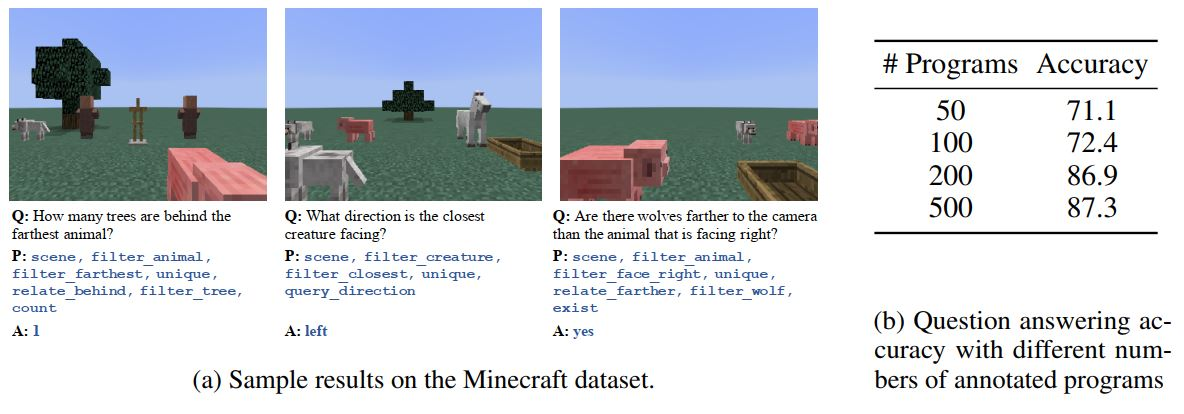
\includegraphics[width=0.9\linewidth]{Fig5.JPG}
    \caption{The model also applies to Minecraft, a world with rich and hierarchical scene context and
    different visual appearance.}
    \label{fig:f5}
\end{figure}

\begin{figure}
    \centering
    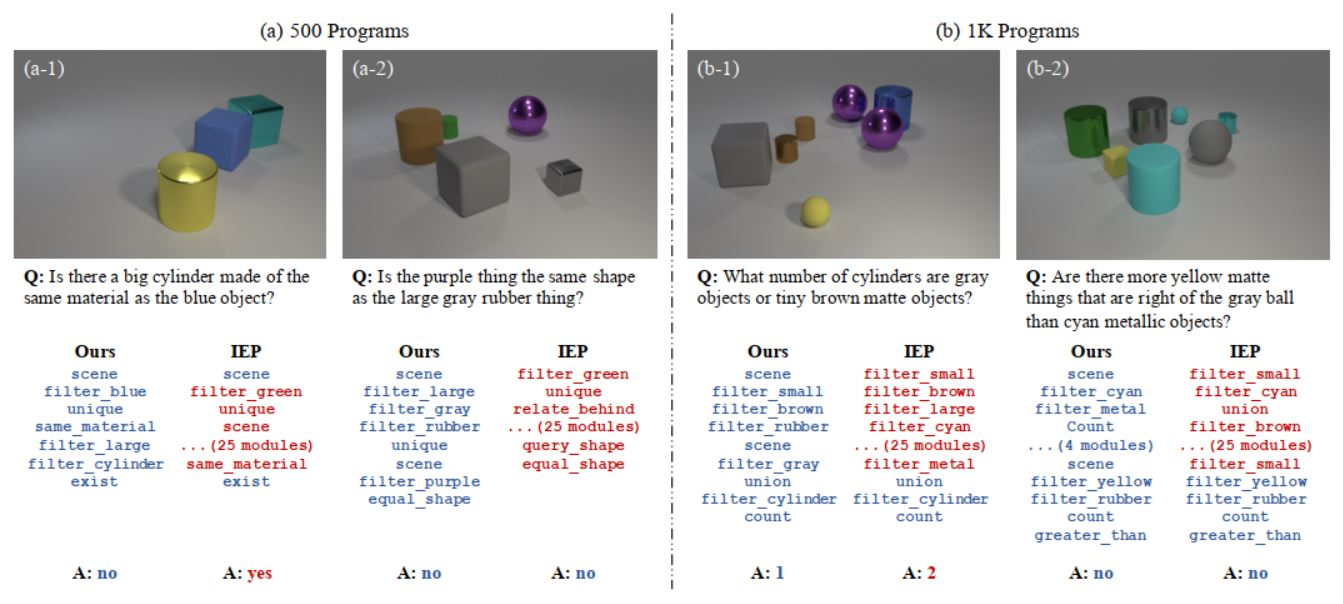
\includegraphics[width=0.9\linewidth]{Fig6.JPG}
    \caption{Qualitative results on CLEVR. Blue color indicates correct program modules and answers;
    red indicates wrong ones. The model is able to robustly recover the correct programs compared to
    the IEP baseline \cite{Johnson2017b}.}
    \label{fig:f6}
\end{figure}

%%

\begin{table}[h!]
    \centering
    \caption{Generalization results on CLEVR-CoGenT.}
    \begin{tabular}{@{}lcccccc@{}}
    \toprule
    Methods & \multicolumn{2}{c}{Not Fine-tuned} & Fine-tune & \multicolumn{2}{c}{Fine-tuned} \\
    \cmidrule(lr){2-3} \cmidrule(lr){5-6}
    & A & B & on & A & B \\
    \midrule
    CNN + LSTM + SA & 80.3 & 68.7 & B & 75.7 & 75.8 \\
    IEP (18K programs) & 96.6 & 73.7 & B & 76.1 & 92.7 \\
    CNN + GRU + FILM & 98.3 & 78.8 & B & 81.1 & 96.9 \\
    TbD + reg & 98.8 & 75.4 & B & 96.9 & 96.3 \\
    NS - VQA (ours) & \textbf{99.8} & 63.9 & B & 64.9 & 98.9 \\
    NS - VQA (ours) & \textbf{99.8} & 63.9 & A + B & \textbf{99.6} & \textbf{99.0} \\
    NS - VQA + Gray (ours) & 99.6 & 98.4 & - & - & - \\
    NS - VQA + Ori (ours) & \textbf{99.8} & \textbf{99.7} & - & - & - \\
    \bottomrule
    \end{tabular}
    \end{table}
    
\begin{table}[h!]
    \centering
    \caption{Question answering accuracy on CLEVR-Humans.}
    \begin{tabular}{@{}lccc@{}}
    \toprule
    \#Programs & NS-VQA & IEP \\
    \midrule
    100 & 60.2 & 38.7 \\
    200 & \textbf{65.2} & 40.1 \\
    500 & \textbf{67.8} & 49.2 \\
    1K & \textbf{67.8} & 63.4 \\
    18K & \textbf{67.0} & 66.6 \\
    \bottomrule
    \end{tabular}
\end{table}

\pagebreak

\section{Conclusion and Future Directions}
The NS-VQA approach represents a significant step towards more robust, interpretable, and data-efficient VQA systems. In summary, this lecture highlights a neuro-symbolic approach to VQA that explicitly separates perception and reasoning. The scene parser extracts a structured representation of the visual scene, while the question parser generates a symbolic program representing the reasoning steps. Training involves a combination of supervised learning and reinforcement learning (REINFORCE) to learn the mapping from questions to executable programs. The results on various datasets demonstrate the model's ability to generalize to novel attribute combinations, human-generated questions, and new visual environments.

Furthermore, CLEVR serves as a valuable diagnostic tool for understanding the strengths and weaknesses of such systems. Future work can explore incorporating explicit short-term memory, encouraging disentangled representations, and developing methods for learning structured representations that generalize to truly novel situations. The combination of deep representation learning with symbolic program execution offers a promising direction for advancing visually grounded language understanding.


\bibliographystyle{plainnat}
\bibliography{references} % references.bib file

\end{document}